\documentclass[10pt,twocolumn]{article}

\usepackage{bold-extra}
\usepackage{color}
\usepackage{epic}
\usepackage{float}
\usepackage{graphicx}
\usepackage{listings}
\usepackage{subfigure}
\usepackage{url}

%%%%%%%%%%%%%%%
%%% Colours %%%
%%%%%%%%%%%%%%%

\definecolor{darkgreen}{rgb}{0, 0.6, 0}
\definecolor{lightgrey}{gray}{0.9}

%%%%%%%%%%%
% Figures %
%%%%%%%%%%%

\newcommand{\stufigex}[5]					% images with specified placement
{
	\begin{figure}[#5]
	\begin{center}
		\includegraphics[#1]{#2}
		\caption{#3}
		\label{#4}
	\end{center}
	\end{figure}
}

% Define the stusubfig environment
\newenvironment{stusubfig}[1]
{
	\begin{figure*}[#1]
	\begin{center}
}
{
	\end{center}
	\end{figure*}
}

%%%%%%%%%%%%%%%%%
% Code Listings %
%%%%%%%%%%%%%%%%%

% Create a new type of float (called a stulisting) for listings
\floatstyle{ruled}
\newfloat{stulisting}{thp}{lop}
\floatname{stulisting}{Listing}

% Setup before using the listings package
\renewcommand{\lstlistingname}{\textbf{Listing}}
\def\thelstlisting{\textbf{\arabic{lstlisting}}}

\lstdefinelanguage{Pseudocode}{
morekeywords={and,assert,break,case,continue,default,down,each,else,for,function,if,not,null,or,rangeswitch,ref,return,switch,then,this,throw,to,up,var,while},
sensitive=true,
morecomment=[l]{//},
morecomment=[s]{/*}{*/}
}

\lstdefinestyle{Default}{
abovecaptionskip=0.5cm,
basicstyle=\scriptsize\ttfamily,
belowcaptionskip=0.5cm,
belowskip=0.5cm,
columns=fixed,
%commentstyle=\color{darkgreen},
commentstyle=\textit, % changed from the thesis (green text looks unprofessional in a journal paper)
language=Pseudocode,
%numbers=left,
numbers=none, % changed from the thesis (line numbers are less relevant here)
numbersep=5pt,
numberstyle=\tiny,
mathescape=true,
showstringspaces=false,
stepnumber=1,
tabsize=4
}

\lstdefinestyle{Snippet}{
abovecaptionskip=0.5cm,
aboveskip=0.5cm,
basicstyle=\small\ttfamily,
belowcaptionskip=0.5cm,
belowskip=0.5cm,
columns=fixed,
commentstyle=\color{darkgreen},
frame=lines,
keywordstyle=\small\bfseries,
language=Pseudocode,
numbers=none,
mathescape=true,
showstringspaces=false,
stepnumber=1,
tabsize=4
}

% For C++ function prototypes
\lstdefinestyle{Prototype}{
abovecaptionskip=0.5cm,
basicstyle=\small\ttfamily,
belowcaptionskip=0.5cm,
belowskip=0.5cm,
columns=fixed,
commentstyle=\color{darkgreen},
language=C++,
numbers=none,
mathescape=true,
showstringspaces=false,
stepnumber=1,
tabsize=4
}

%%%%%%%%%%%%%%%%%
% Main Document %
%%%%%%%%%%%%%%%%%

\begin{document}

\title{Object-Environment Collision Detection using Onion BSPs}
\author{Stuart Golodetz}
\date{}
\maketitle

\section{Introduction}

In my last article \cite{golodetzoverload13oct}, I described how to automatically generate navigation meshes to support the navigation of agents around 3D environments (e.g.~game worlds), as implemented in my homemade \emph{hesperus} engine \cite{hesperus}. However, there is far more to such navigation than simply mesh generation: it remains to be shown how to determine where (if anywhere) an agent can be found on the mesh and how to make best use of the mesh when allowing both user-controlled and AI agents to move around the environment. Agent movement must necessarily interact with an implementation's physics system, since the navigation mesh only covers the \emph{walkable} surfaces of the world and there is a need to ensure that agents are simulated correctly even when they are not on the mesh. In particular, any implementation needs to ensure that agents do not collide with either the world or each other, and that the effects of forces such as gravity are properly applied to them when not on the mesh. For that reason, before tackling the agent movement problem itself, it is important to take a step back and look at how to implement a simple physics system.

As a first step to describing how the physics system in \emph{hesperus} works, I want to focus this article on a way of detecting collisions between objects (including agents) and their environment, via the construction of a special binary space partitioning (BSP) representation of the world that I call an \emph{onion BSP} (for reasons that will become obvious). Future articles will focus on how to detect object-object collisions using a technique called Minkowski Portal Refinement \cite{snethen08}, and how to combine the techniques into a rudimentary physics system, before we return to the original problem of agent movement. Readers who are interested in a more general look at games physics engine development are advised to take a look at the excellent (and aptly-named) book by Millington on the topic \cite{millington07}.

The organisation of this article is as follows: in \S\ref{sec:bsps}, I briefly review the ideas behind binary space partitioning (readers may wish to take a look back at a previous article I wrote for more details \cite{golodetzoverload08aug}); in \S\ref{sec:onionbsps}, I describe how to construct onion BSPs, an extension of BSP trees for multiple configuration spaces, based on the approach of van Waveren in \cite{vanwaveren01}; in \S\ref{sec:collisiondetection}, I describe how to perform continuous collision detection between objects and onion BSPs using an algorithm for finding the first point at which a half-ray crosses a wall in the world; and in \S\ref{sec:conclusions} I conclude.

\section{Binary Space Partitioning}
\label{sec:bsps}

In its most general form, binary space partitioning is a technique for representing n-dimensional space as a binary tree (known as a BSP tree) by recursively dividing it into two using \emph{hyperplanes} (the n-dimensional generalisation of planes). For a 2D example, see Figure~\ref{?}. Each node of a BSP tree represents a convex subspace of the world being partitioned (see Figure~\ref{?}). Branch nodes have an associated split plane (a line with facing in 2D) that divides the subspace represented by the node in two. Each leaf node contains the polygons (line segments in 2D) that fall within the subspace it represents.

Binary space partitioning was originally introduced by Fuchs et.\ al \cite{fuchs80} in 1980. It saw widespread use in first-person games of the \emph{Quake} era (e.g.~see \cite{abrash97}) as a way of representing 3D game worlds, most notably because it provided a way of rendering a world's polygons in either back-to-front or front-to-back order without the need for a z-buffer on the graphics card (z-buffers once used to be quite costly). As graphics cards have matured, commercial games have moved away from binary space partitioning as a rendering approach, because traversing a BSP tree is relatively slow in comparison to simply throwing large numbers of triangles at the graphics card and letting the z-buffer handle the rendering order, but BSP trees remain interesting as a basis for collision detection.

TODO: Briefly explain BSP construction

\section{Onion BSPs}
\label{sec:onionbsps}

TODO: Explanation of onion BSPs in terms of configuration spaces

%---
\begin{stusubfig}{!t}
	\subfigure[]
	{
	\begin{picture}(250,50)
		\thicklines
		\dashline{4}(0,35)(35,35)
		\dashline{4}(0,165)(35,165)
		\dashline{4}(215,165)(250,165)
		\dashline{4}(215,25)(215,0)
		\dashline{4}(35,75)(75,75)
		\dashline{4}(175,75)(215,75)
		\dashline{4}(35,125)(75,125)
		\dashline{4}(175,125)(215,125)
		\put(122.5,180){a}
		\put(230,97.5){b}
		\put(122.5,15){c}
		\put(15,97.5){d}
		\put(122.5,140){e}
		\put(190,97.5){f}
		\put(122.5,57.5){g}
		\put(57.5,97.5){h}
		\put(122.5,97.5){i}

		\color{red}
		\put(35.4,35.4){\framebox(179.2,129.2){}}
		\put(125,35){\vector(0,1){10}}		\put(130,37.5){2}
		\put(125,165){\vector(0,-1){10}}	\put(130,155){0}
		\put(35,100){\vector(1,0){10}}		\put(37.5,105){3}
		\put(215,100){\vector(-1,0){10}}	\put(207.5,105){1}
		\color{green}
		\put(75.4,75.4){\framebox(99.2,49.2){}}
		\put(125,75){\vector(0,1){10}}		\put(130,77.5){6}
		\put(125,125){\vector(0,-1){10}}	\put(130,115){4}
		\put(75,100){\vector(1,0){10}}		\put(77.5,105){7}
		\put(175,100){\vector(-1,0){10}}	\put(167.5,105){5}
		\color{black}
	\end{picture}
	}
	%
	\hspace{12mm}%
	%
	\subfigure[]
	{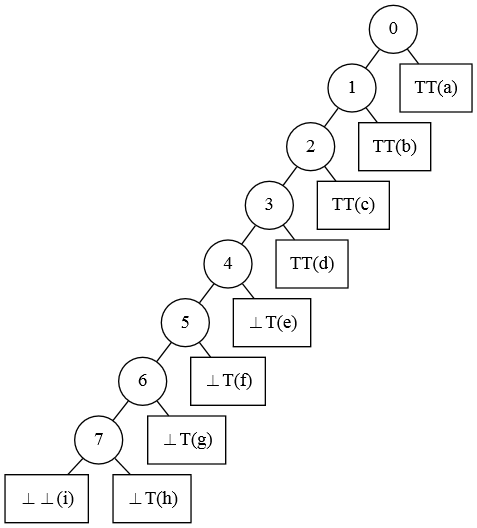
\includegraphics[width=.35\linewidth]{onion-example.png}}%
\caption{TODO}
\label{fig:onion-example}
\end{stusubfig}
%---

\subsection{The Compilation Process}

Onion BSP compilation is in principle much the same as BSP compilation (see \cite{golodetzoverload08aug}), but slightly trickier because we have to test the solidity of each leaf in each configuration space rather than getting it for free as part of the compilation process. An explanation of this testing process is deferred to the next section, but it also has an impact on the main part of the compilation. In particular, the test involves checking an arbitrary point in the leaf for solidity in each configuration space (the solidity of any point in the leaf is guaranteed to be the same as that of the entire leaf), so we will need (a) a way of determining an arbitrary point in a leaf, and (b) a way of testing a point for solidity in a configuration space. As will be seen, determining an arbitrary point in a leaf will involve knowing the set of split planes on the path from the root of the tree to the leaf, so these should be maintained during compilation. To test a point's solidity in a configuration space, we build a normal BSP tree for the space at the start of the compilation process and later classify the point with regard to it. To determine a full solidity vector for a leaf, we have to test the leaf's arbitrary point against each such BSP tree in turn.

The resulting main compilation process is shown in Listings~\ref{code:build-tree} and \ref{code:build-subtree}. The key thing to note is the way in which a set of split planes is maintained in order to facilitate solidity testing -- we add the current split plane to the set before each recursive call to \texttt{build\_subtree} and remove it again afterwards, so that whenever we reach a leaf it will contain precisely those split planes on the path from the root of the tree to the leaf. Note that orientation is important, so the current split plane must be reversed when recursing into the right-hand subtree.

%---
\begin{stulisting}[!t]
\caption{Building an Onion Tree}
\label{code:build-tree}
\lstinputlisting[style=Default]{build-tree.lst}
\end{stulisting}
%---

%---
\begin{stulisting}[!t]
\caption{Building an Onion Subtree}
\label{code:build-subtree}
\lstinputlisting[style=Default]{build-subtree.lst}
\end{stulisting}
%---

\subsection{Determining Leaf Solidity}

TODO

%---
\begin{stulisting}[!t]
\caption{Determining Leaf Solidity}
\label{code:determine-leaf-solidity}
\lstinputlisting[style=Default]{determine-leaf-solidity.lst}
\end{stulisting}
%---


\section{Collision Detection}
\label{sec:collisiondetection}

TODO

\section{Conclusions}
\label{sec:conclusions}

TODO

\section{Acknowledgements}

TODO

%
% Detecting Object-Object Collisions using Minkowski Portal Refinement
% A Simple Physics Engine for 3D Games
% Agent Localisation and Movement in 3D Environments
%

\clearpage

%\nocite{*}

\bibliographystyle{plain}
\bibliography{onionbsp}

\end{document}